
 \let\negmedspace\undefined
\let\negthickspace\undefined
\documentclass[journal]{IEEEtran}
\usepackage[a5paper, margin=10mm, onecolumn]{geometry}
%\usepackage{lmodern} % Ensure lmodern is loaded for pdflatex
\usepackage{tfrupee} % Include tfrupee package

\setlength{\headheight}{1cm} % Set the height of the header box
\setlength{\headsep}{0mm}     % Set the distance between the header box and the top of the text
\usepackage{gvv-book}
\usepackage{gvv}
\usepackage{cite}
\usepackage{amsmath,amssymb,amsfonts,amsthm}
\usepackage{algorithmic}
\usepackage{graphicx}
\usepackage{textcomp}
\usepackage{xcolor}
\usepackage{txfonts}
\usepackage{listings}
\usepackage{enumitem}
\usepackage{mathtools}
\usepackage{gensymb}
\usepackage{comment}
\usepackage[breaklinks=true]{hyperref}
\usepackage{tkz-euclide} 
\usepackage{listings}
% \usepackage{gvv}                                        
\def\inputGnumericTable{}                                 
\usepackage[latin1]{inputenc}                                
\usepackage{color}                                            
\usepackage{array}                                            
\usepackage{longtable}                                       
\usepackage{calc}                                             
\usepackage{multirow}                                         
\usepackage{hhline}                                           
\usepackage{ifthen}                                           
\usepackage{lscape}



\usepackage{amsmath,amssymb}
\usepackage{booktabs}
\usepackage{tikz}
\usetikzlibrary{arrows.meta,angles,quotes}





\begin{document}

\bibliographystyle{IEEEtran}
\vspace{3cm}

\title{2.6.32}
\author{AI25BTECH11021 - Abhiram Reddy N}
% \maketitle
% \newpage
% \bigskip
{\let\newpage\relax\maketitle}

\renewcommand{\thefigure}{\theenumi}
\renewcommand{\thetable}{\theenumi}
\setlength{\intextsep}{10pt} % Space between text and floats


\numberwithin{equation}{enumi}
\numberwithin{figure}{enumi}
\renewcommand{\thetable}{\theenumi}


\section*{\textbf{Question 2.6.32}}

Find the area of the triangle whose vertices are 
\[
(1, -1), \quad (-4, 6), \quad (-3, 5).
\]

\section*{\textbf{Solution}}

\subsection*{Step 1: Define the vertices as vectors}
\[
A = \begin{pmatrix} 1 \\ -1 \end{pmatrix}, \quad
B = \begin{pmatrix} -4 \\ 6 \end{pmatrix}, \quad
C = \begin{pmatrix} -3 \\ 5 \end{pmatrix}
\]

\subsection*{Step 2: Calculate the vectors \( A - B \) and \( B - C \)}
\[
A - B = \begin{pmatrix} 1 \\ -1 \end{pmatrix} - \begin{pmatrix} -4 \\ 6 \end{pmatrix} 
= \begin{pmatrix} 5 \\ -7 \end{pmatrix}
\]

\[
B - C = \begin{pmatrix} -4 \\ 6 \end{pmatrix} - \begin{pmatrix} -3 \\ 5 \end{pmatrix} 
= \begin{pmatrix} -1 \\ 1 \end{pmatrix}
\]

\subsection*{Step 3: Calculate the 2D cross product magnitude}
For vectors \(\mathbf{u} = \begin{pmatrix} u_1 \\ u_2 \end{pmatrix}\) and \(\mathbf{v} = \begin{pmatrix} v_1 \\ v_2 \end{pmatrix}\), the 2D cross product is
\[
\mathbf{u} \times \mathbf{v} = u_1 v_2 - u_2 v_1.
\]

Applying this,
\[
(A-B) \times (B-C) = 5 \times 1 - (-7) \times (-1) = 5 - 7 = -2
\]

\[
\Rightarrow \| (A-B) \times (B-C) \| = 2
\]

\subsection*{Step 4: Calculate the area of the triangle}
\[
ar(ABC) = \frac{1}{2} \times \| (A-B) \times (B-C) \| = \frac{1}{2} \times 2 = 1
\]

\[
\boxed{ar(ABC) = 1 \text{ square unit}}
\]


\begin{figure}[htbp]
\centering
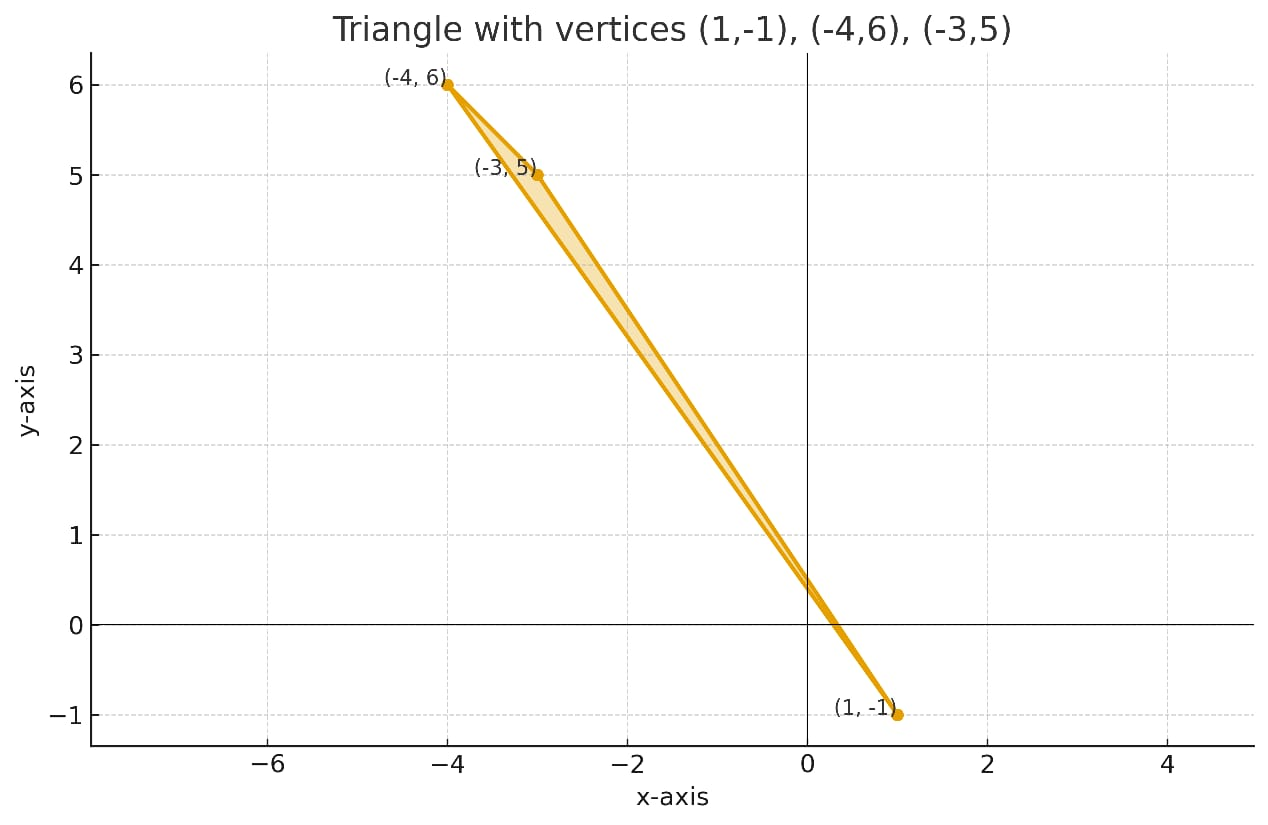
\includegraphics[width=0.8\columnwidth]{figs/python_plot.png} 
\caption{plot}
\label{fig:1}
\end{figure}



\end{document}